\nsection{OSN 5 Образцы (паттерны) проектирования, их классификация и способ описания. Примеры образцов: структурного, поведенческого и порождающего.}

Образец (или паттерн) – это типовое проектное решение конкретной задачи проектирования, описанное специальным образом, чтобы облегчить его повторное применение. Фактически, каждый паттерн является формализованным опытом лучших разработчиков в индустрии создания ПО. Основные составляющие части описания образца: Имя. Идентифицирует образец. Хорошее имя характеризует решаемую проблему и способ ее решения. Задача. Описание ситуации, в которой следует применять образец. Это описание включает в себя: постановку проблемы, контекст проблемы, перечень условий, при выполнении которых имеет смысл применять образец. Решение. Описание элементов архитектуры, связей между ними, функций каждого элемента. Включает в себя UML-диаграммы. Результаты. Следствия применения паттерна и компромиссы. Преимущества и недостатки образца. Влияние использования образца на гибкость, расширяемость и переносимость системы. 3 типа: порождающие образцы (способы создания экземпляров классов); структурные образцы (способы задания статических связей между проектными классами); образцы поведения (способы организации взаимодействий между объектами).

\textbf{Мост (Bridge) Классификация: структурный образец.}
Назначение: отделить абстракцию от реализации.
Мотивация: наследование жестко привязывает реализацию к абстракции, поэтому лучше иметь иерархию наследования для интерфейсов и отдельно их реализации.
Пример: Пусть есть абстракция Shape (форма), в ней есть операция draw(), отвечающая за отрисовку. В каждой конкретной форме (Rectangle, Circle) отрисовка реализуется с помощью примитивов drawLine(), drawCircle(), описанных в интерфейсе Drawing, реализуемом разными графическими утилитами DrawingV1, DrawingV2, рассчитанными на работу с разными графическими устройствами Driver1, Driver2. Диаграмма классов:
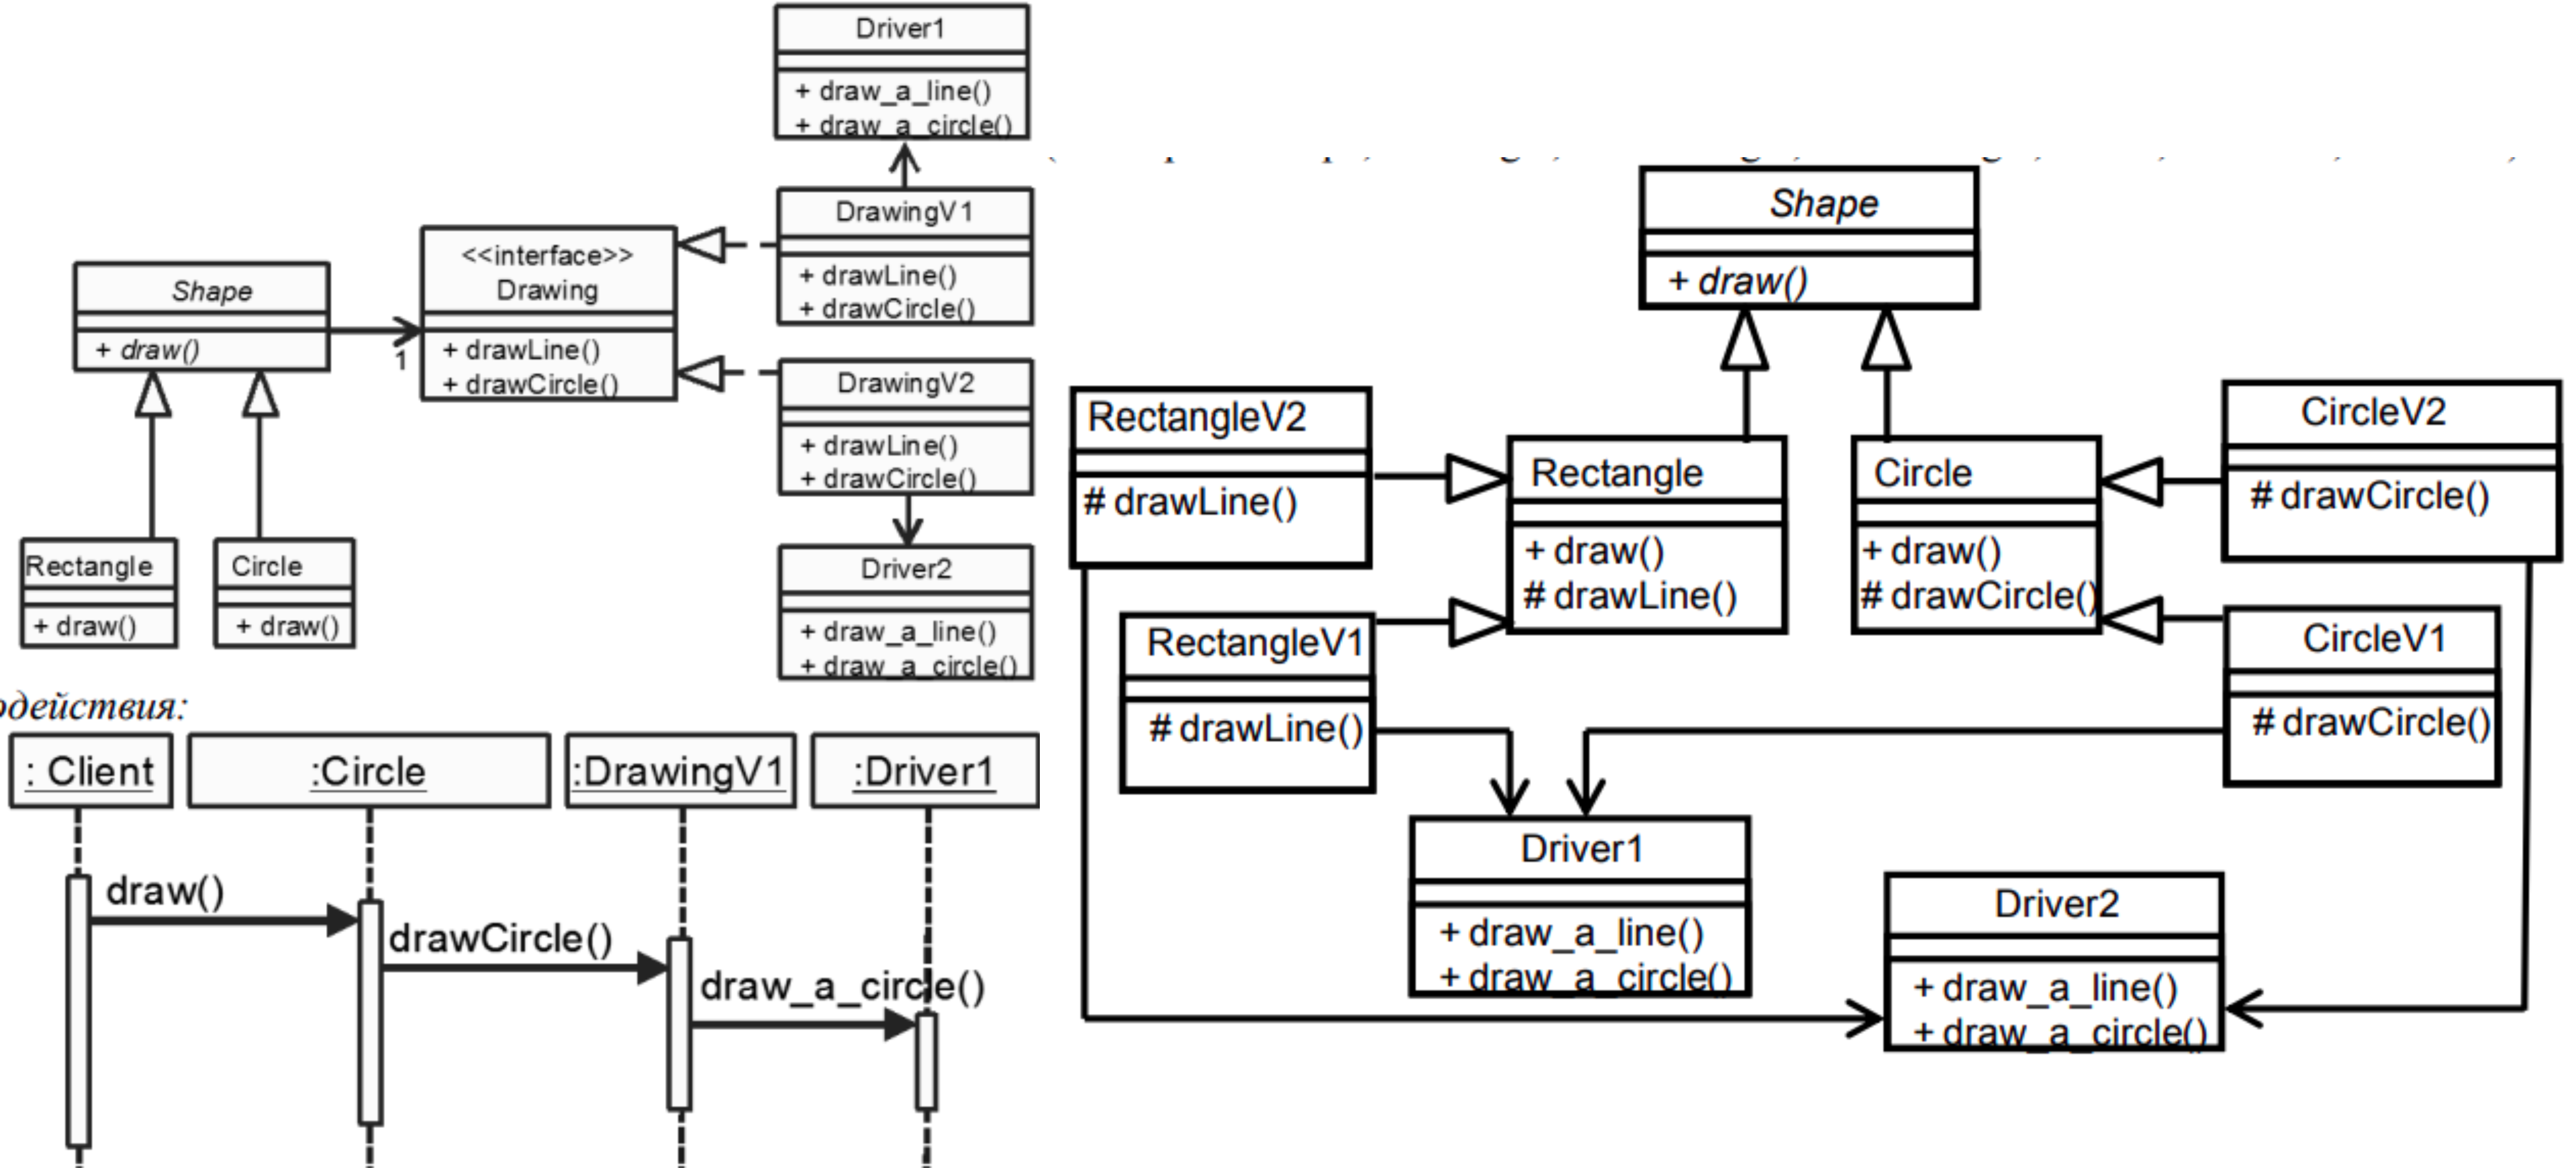
\includegraphics[scale=0.055]{pics/5_1.png}
Если не применять образец, то у Rectangle и Circle могли бы быть два наследника, каждый из которых рассчитан на работу с одним из двух вариантов графики. Т. е. в иерархии форм было бы 7 классов (см на рис.: Shape, Rectangle, V1Rectangle, V2Rectangle, Circle, V1Circle, V2Circle).Если добавить ещё формы – наследницы Shape – Triangle, PolyLine, то в первом случае при их отрисовке дополнительные классы не нужны, так как можно воспользоваться реализациями Drawing. Во втором случае иерархия разрастается, в ней становится 13 классов (добавляются Triangle, TriangleV1, TriangleV2, PolyLine, PolyLineV1, PolyLineV2). Аналогично применение паттерна Мост выгодно при добавлении поддержки еще одного графического устройства Driver3. Будет достаточно добавить новую реализацию интерфейса Drawing – класс DrawingV3, вместо того, чтобы заводить каждой конкретной фигуре наследника с реализацией отрисовки для нового устройства (RectangleV3, CircleV3, TriangleV3, PolyLineV3).

\textbf{Strategy (Стратегия) Классификация: образец поведения.} Назначение: Определяет семейство алгоритмов, инкапсулирует каждый из них и делает их взаимозаменяемыми. Мотивация: есть несколько алгоритмов решения одной задачи, которые нежелательно «зашивать» в клиентский класс. Результаты: 1 Иерархия классов стратегий определяет семейство алгоритмов или поведений, которые можно повторно использовать. 2 Инкапсуляция алгоритма в отдельный класс позволяет изменять его независимо от контекста. 3 Избавляемся от if и switch (улучшаем читаемость кода). Приведем пример использования образца для реализации разных стратегий расчета налогов:

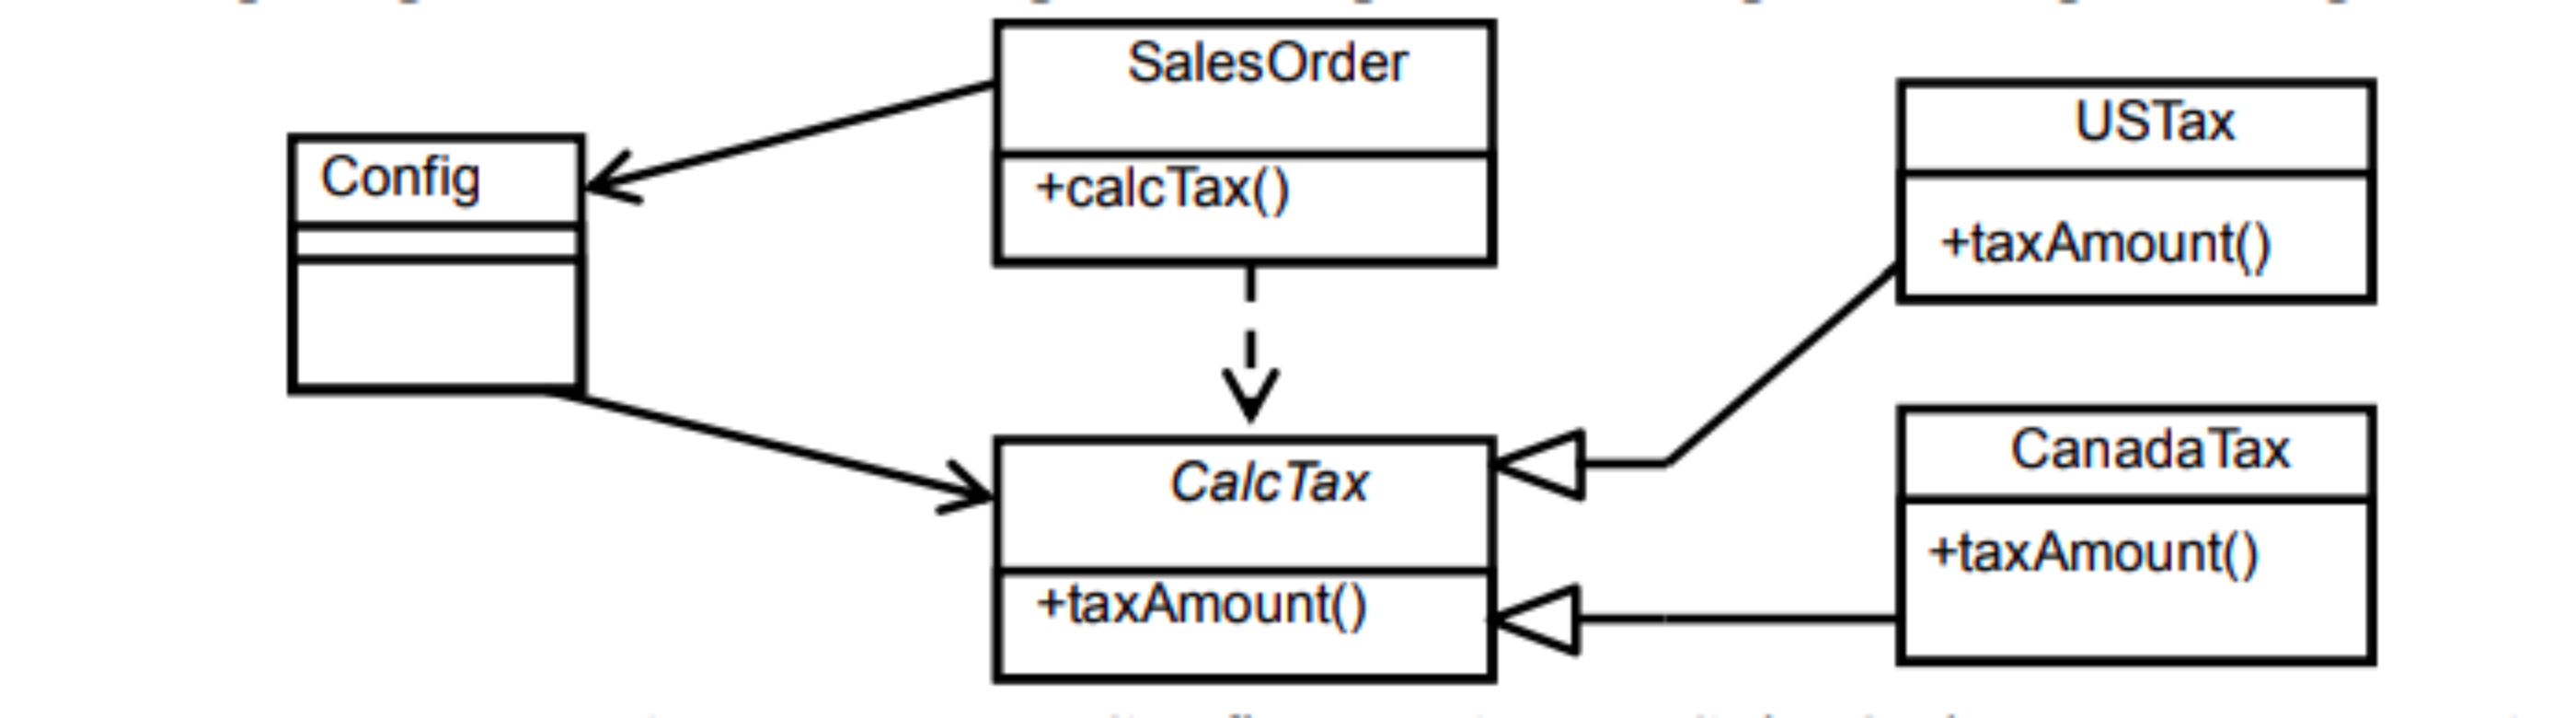
\includegraphics[scale=0.07]{pics/5_2.png}

Предполагается, что объект класса Config сообщает SalesOrder ссылку на объект-алгоритм расчета налогов (либо экземпляр USTax, пригодный для США, либо CanTax, пригодный для Канады). Если потребуется добавить новые способы расчета, достаточно добавить подклассы CalcTax. Обратите внимание, что в примере вместо интерфейса и реализации используется абстрактный класс и связи обобщения. Альтернативой предложенному решению является внесение внутрь SalesOrder::calcTax() логики выбора схемы расчета и реализация расчетов в отдельных операциях SalesOrder. Модифицируемость такого решения ниже, чем при использовании образца.

\textbf{Абстрактная фабрика (Abstract Factory) Классификация: образец порождения объектов.} Назначение: предоставляет интерфейс для создания взаимосвязанных и взаимозависимых объектов, не определяя их конкретных классов. Мотивация: часто встает задача проектирования программной системы независимой от конкретной реализации GUI. Результаты:
\begin{enumerate}
    \item изоляция клиента от деталей реализации классов-продуктов (их имена известны только конкретной фабрике);
    \item упрощение замены семейств продуктов;
    \item набор классов-продуктов фиксирован, добавлять новые продукты в семейства трудно
\end{enumerate}

Представим, что нужно добавить третий класс продуктов. Потребуется добавить иерархию из 3-х классов и дополнительный метод в каждую фабрику, что довольно затратно. Пример: две фабрики обеспечивают производство семейств классов-драйверов, работающих с низким или высоким разрешением. Предполагается, что разрешение драйвера принтера должно соответствовать дисплейному.

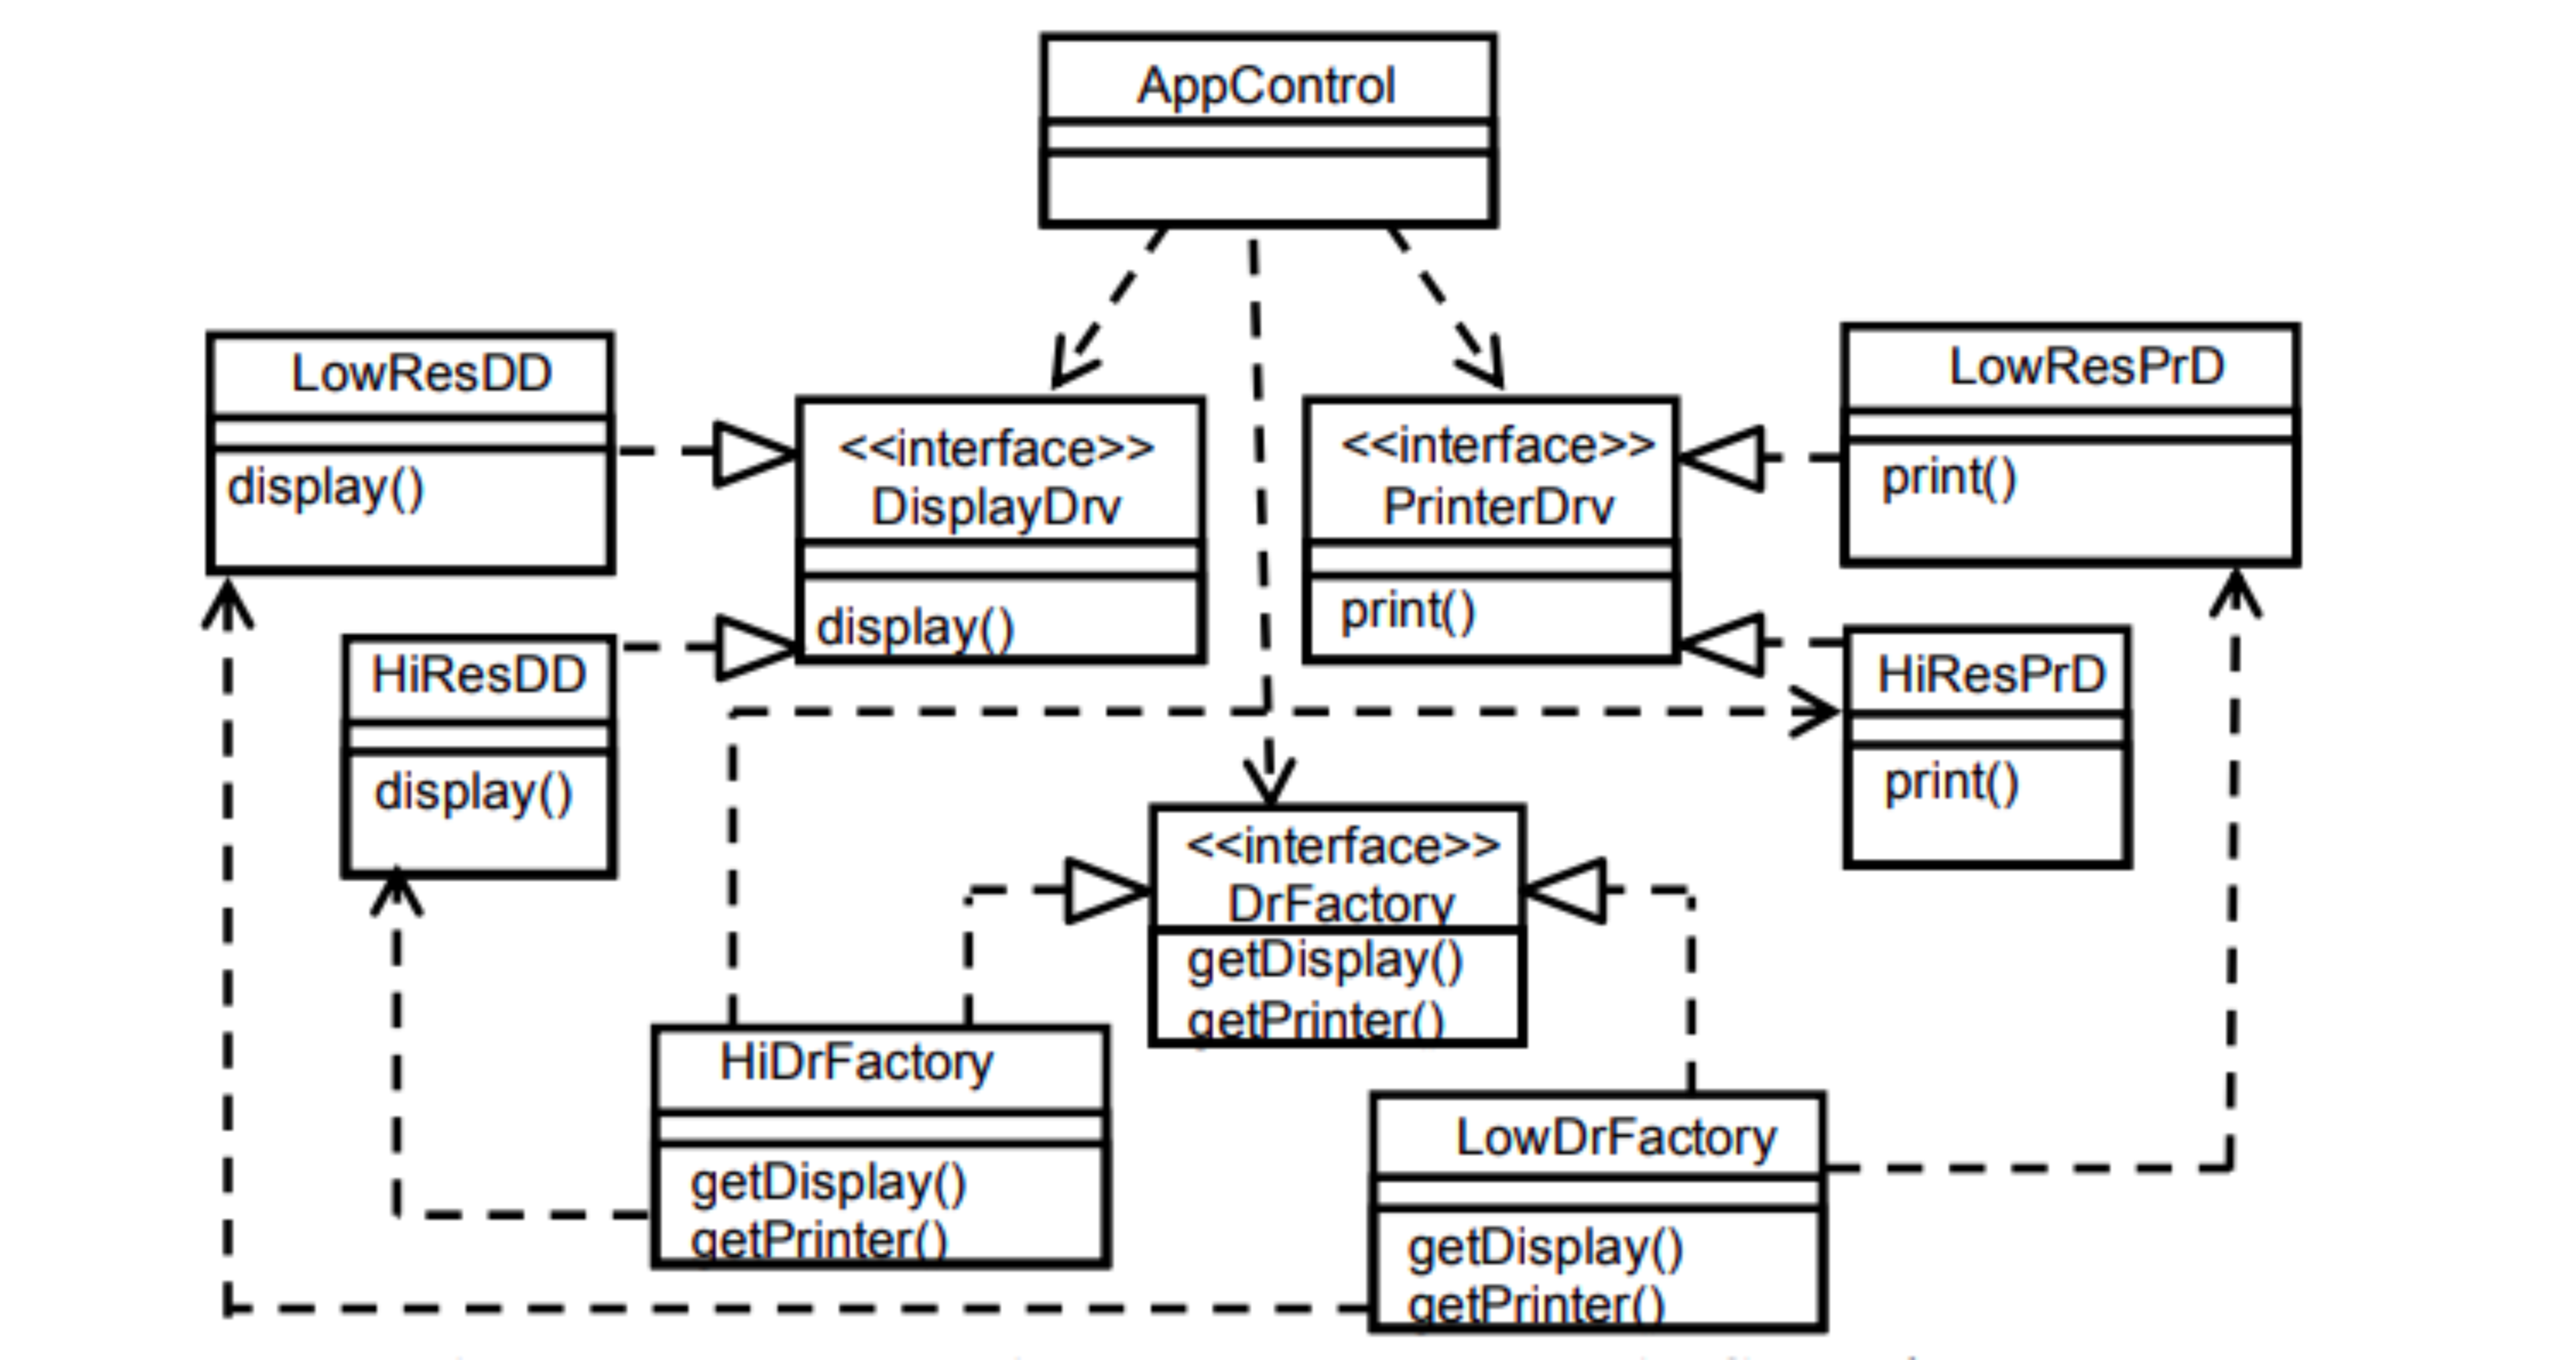
\includegraphics[scale=0.08]{pics/5_3.png}

Без применения образца пришлось бы связывать класс AppControl прямыми зависимостями с классами LowResDD, HiResDD, LowResPrD, HiResPrD. На диаграмме, приведённой выше, предполагается, что классы LowResPrD и HiResPrD могут иметь общий интерфейс (или общий суперкласс).